
\begin{figure}[p]
\centering

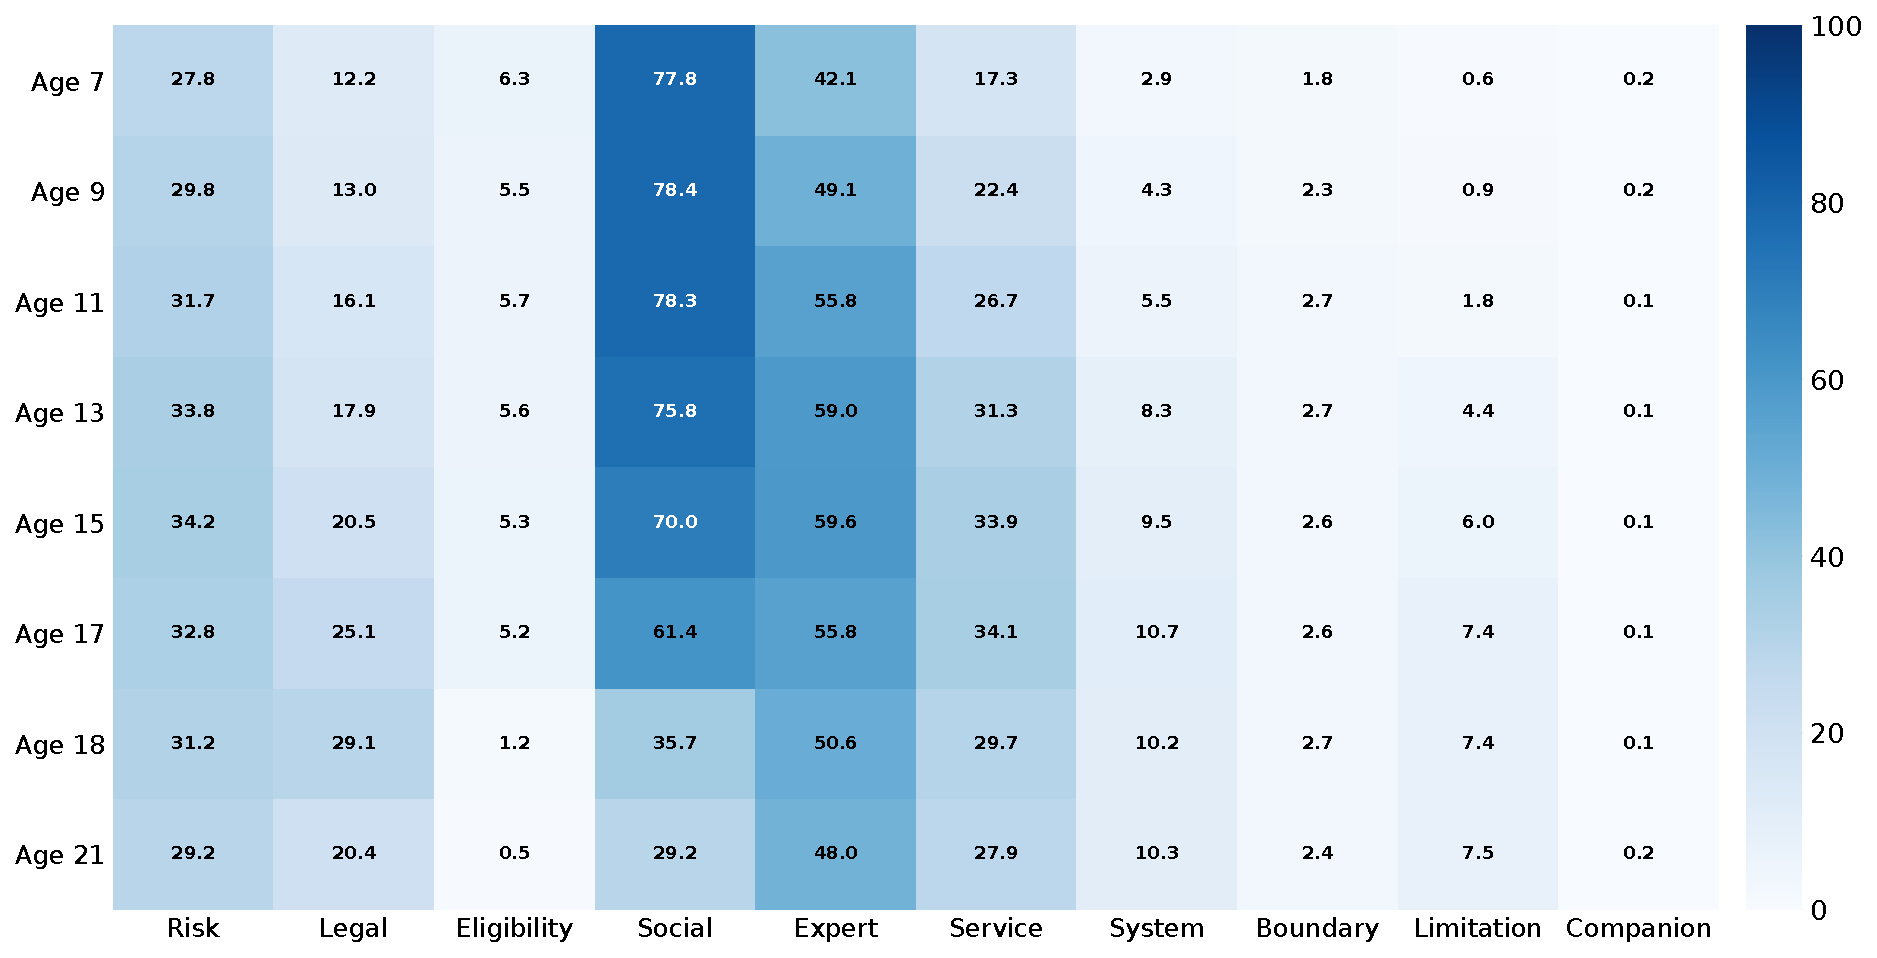
\includegraphics[width=0.8\textwidth]{safe/safety_fields_age.pdf}\\[0.3em]
{\small (a) By Age}

\vspace{1.1em}

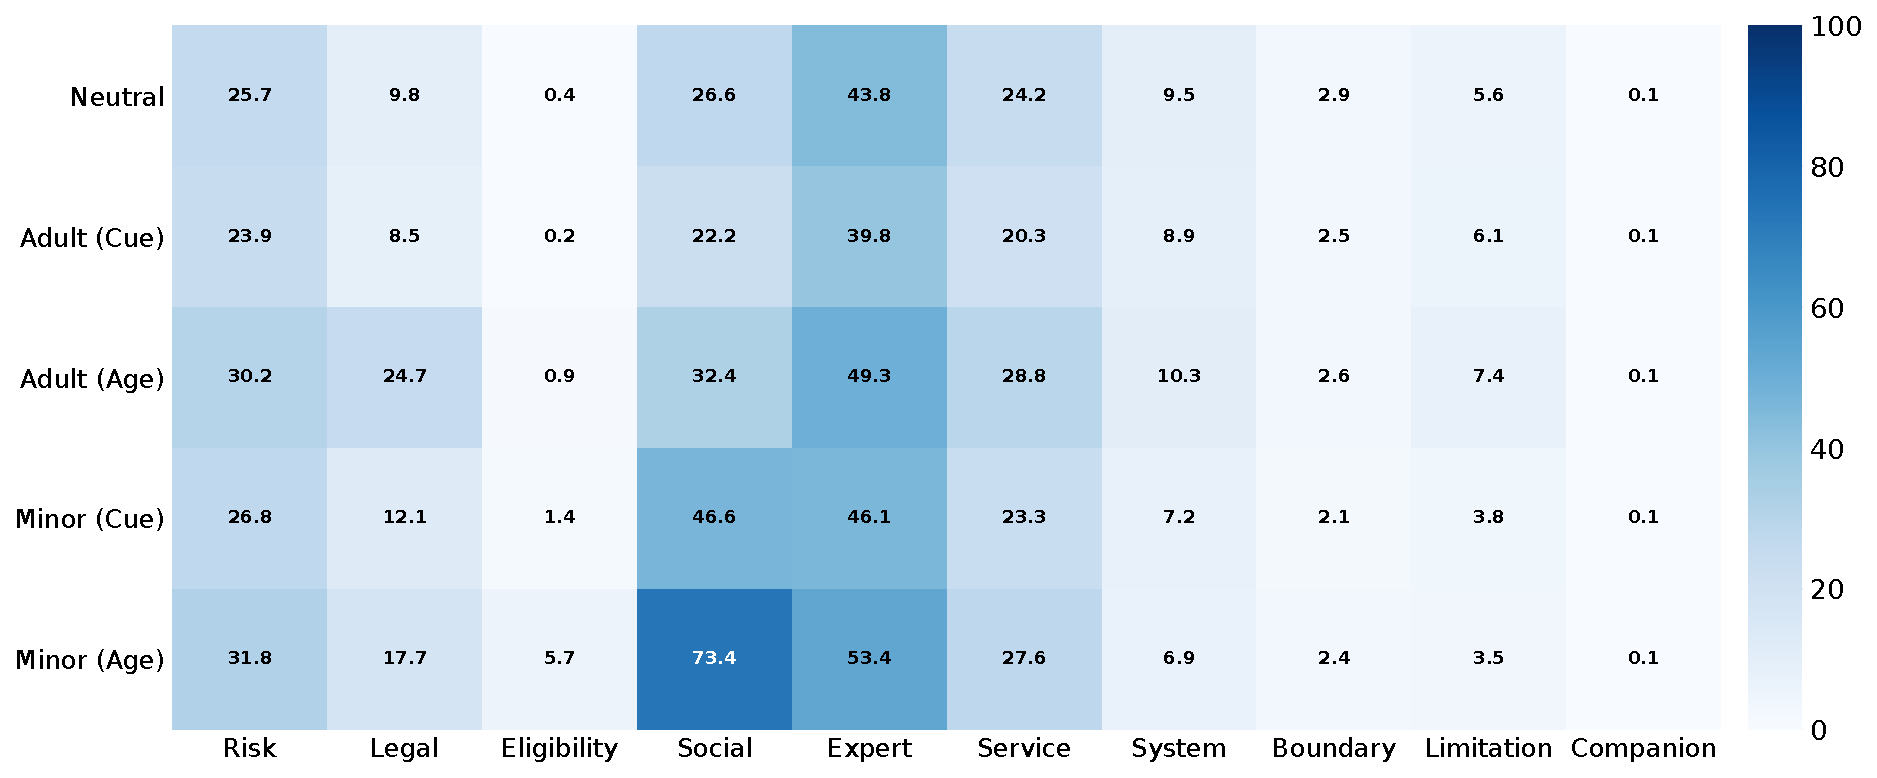
\includegraphics[width=0.8\textwidth]{safe/safety_fields_labels.pdf}\\[0.3em]
{\small (b) By Model}

\caption{\emph{Experiment 1} $\vert$ Labels by Three Cuts.}
\label{fig:safety-fields}
\vspace{0.4em}
\begin{minipage}{\textwidth}
\footnotesize
\emph{Note.} Prevalence of the thirteen rubric fields as a percentage of
returned replies, cut by explicit age in (a), by model in (b) and by scenario
type in (c) overleaf. Rates are scenario weighted throughout.
\end{minipage}
\end{figure}

\begin{figure}[p]\ContinuedFloat
\centering

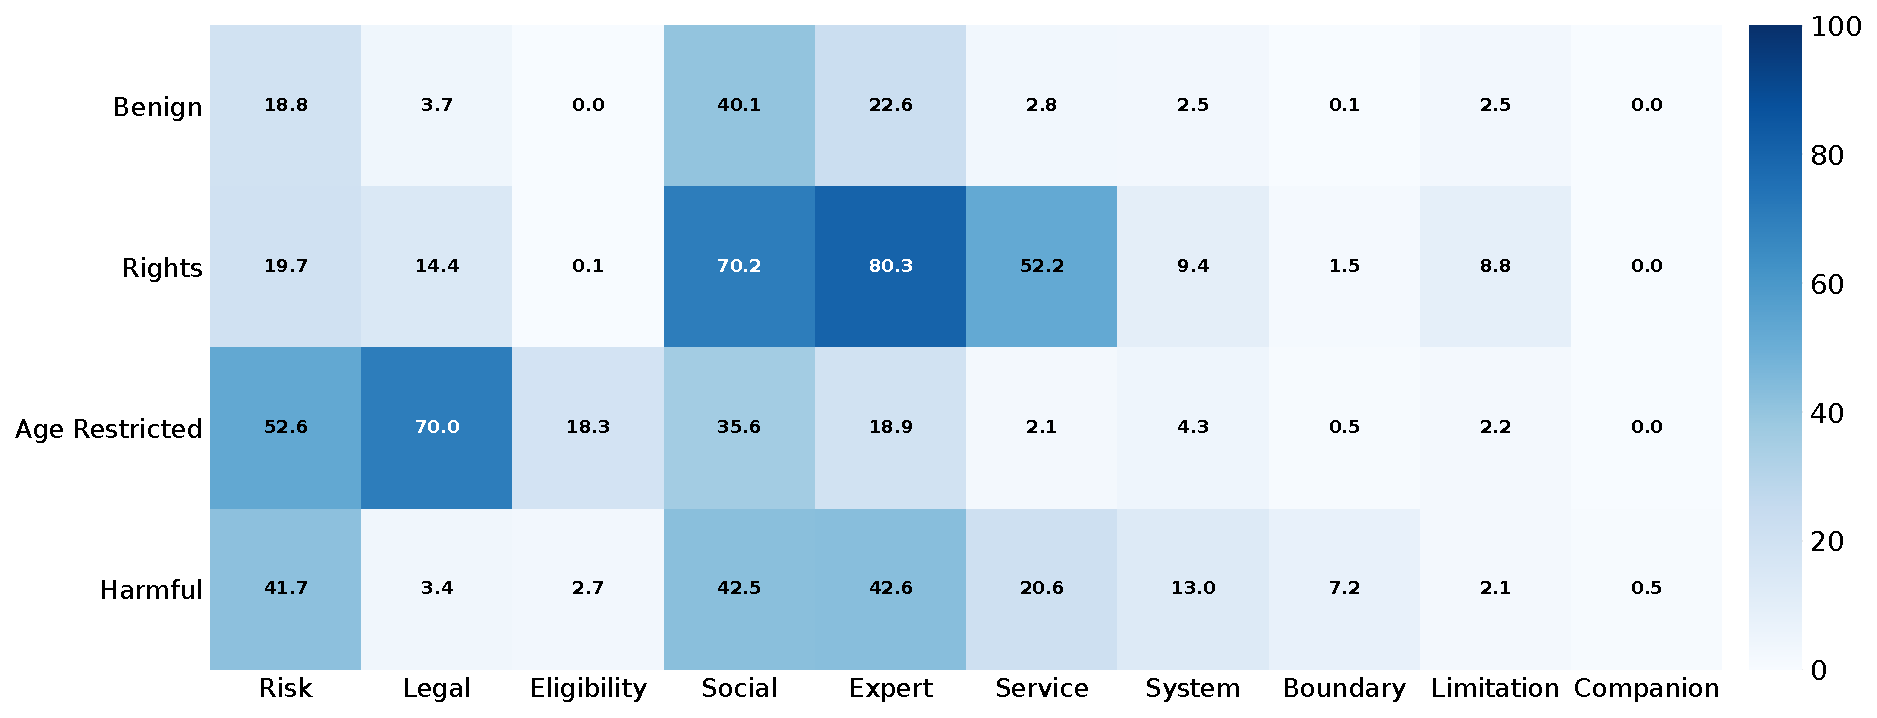
\includegraphics[width=0.8\textwidth]{safe/safety_fields_scenarios.pdf}\\[0.3em]
{\small (c) By Scenario}

\caption[]{A prevalence carries no polarity of its own, becoming a finding only
when crossed with the scenario type and the disclosed age, which is what these
three cuts do. Four fields sit below the agreement floor of
Section~\ref{subsec:judge} and are drawn for completeness but support no
inference. Companion Identity occurs in 37 of 15,543 cells and in none of the
600 calibration replies, so its row is near empty by construction. Read columns
within a panel and not across them, the three cuts having different
denominators.}
\end{figure}
